\documentclass{article}
\usepackage{graphicx} % Required for inserting images
\usepackage{float}
\usepackage[T1]{fontenc}
\usepackage{amsmath}
\usepackage[margin=1in]{geometry}
\usepackage{booktabs}
\usepackage{tabularx}
\usepackage[hidelinks]{hyperref}

\title{Selling 25-delta puts instead of ATM puts on the short-only book}
\author{Experiment report \textperiodcentered{} L/S Gamma Desk, QUANTT}
\date{2026-10-17}

\begin{document}

\maketitle

\textbf{Question:} On the short-only book with the 10-share hedge band, does selling a put near 25 delta instead of the ATM put raise net P\&L at 1x and 2x spreads, in both halves, without a worse daily tail?

\textbf{Method:}

\begin{itemize}

\item \textbf{Pre-registration:} the hypothesis card was committed before any run (commit 06dbdc8). The research-only engine switch was committed just before it (ca37360).

\item \textbf{Data:} the paper rules (\texttt{configs/\allowbreak{}paper.\allowbreak{}toml}), with the changes below, are replayed on R2 replay snapshots v1 (config\_hash b040760187f0) over the development window 2014-06-02 to 2024-12-31. The hold-out (2025-01-01 to 2026-07-10) was not used.

\item \textbf{Book:} short-only (\texttt{long\_\allowbreak{}band = -\allowbreak{}inf}) with the 10-share hedge band (\texttt{min\_\allowbreak{}shares = 10}), the best book so far. The signal is unchanged: VRP on the ATM IV of the chosen \textasciitilde{}30-DTE expiry against the GARCH forecast, short above +2 vol points. Exits and hedges run once a day at 10:15 ET.

\item \textbf{New, research-only switch:} \texttt{[backtest] put\_\allowbreak{}delta} (default 0 = ATM, as live). When it is set, the engine sells the put on the same expiry whose |delta| is closest to the target. With the switch off, the engine reproduces baseline trial 1 exactly.

\item \textbf{Variants:} \texttt{put25} (primary, 25 delta) and \texttt{put35} (sensitivity, 35 delta, reported only).

\item \textbf{Reference:} the registered runs of \texttt{2026-\allowbreak{}10-\allowbreak{}16-\allowbreak{}short-\allowbreak{}only-\allowbreak{}band10/\allowbreak{}band10}, reused and not rerun. Their strategy config is identical apart from the strike.

\item \textbf{Runs:} every variant ran once at 1x and 2x spreads. Costs are \$0.65 per contract and \$0.005 per share, with a \$1 minimum per order.

\end{itemize}

This report was written by Claude at the PM's request.

\section{Result vs the pass bar}

\texttt{put25} against \texttt{band10} at the same spread multiple. P\&L is net USD on daily equity for 1 contract. ES is the mean of the worst 5\% of daily P\&L.

\begin{center}\small
\begin{tabularx}{\linewidth}{>{\raggedright\arraybackslash}X l l l l >{\raggedright\arraybackslash}X}
\toprule
\textbf{Check} & \textbf{1x value} & \textbf{1x bar} & \textbf{2x value} & \textbf{2x bar} & \textbf{Result} \\
\midrule
Net P\&L, full window & +180 & > \ensuremath{-}170 & \ensuremath{-}273 & > \ensuremath{-}1,847 & pass \\
Net P\&L, 2014-06 to 2019-12 & \ensuremath{-}280 & > \ensuremath{-}691 & \ensuremath{-}410 & > \ensuremath{-}1,180 & pass \\
Net P\&L, 2020-01 to 2024-12 & +460 & > +521 & +137 & > \ensuremath{-}667 & \textbf{fail 1x}, pass 2x \\
abs ES 5\% \ensuremath{\leq} 1.10 \ensuremath{\times} reference & 72.0 & \ensuremath{\leq} 96.2 & 73.2 & \ensuremath{\leq} 104.8 & pass \\
Event floor: round trips (1x) & 105 & \ensuremath{\geq} 30 &  &  & met \\
\bottomrule
\end{tabularx}
\end{center}

\textbf{Verdict: failed}, on one of eight checks: 2020-2024 at 1x, by \$60 (+\$460 against +\$521). Every other check passes, most by a wide margin. This is still the first book in the desk's backtests with positive net P\&L over the full window at 1x (+\$180). At 2x it is close to flat (\ensuremath{-}\$273). It also has the smallest maximum drawdown in the desk's backtests, and a smaller daily tail than the reference.

\subsection{Full-window numbers (not part of the bar)}

\begin{center}\small
\begin{tabularx}{\linewidth}{>{\raggedright\arraybackslash}X l l l l l l}
\toprule
\textbf{} & \textbf{band10 1x} & \textbf{put25 1x} & \textbf{put35 1x} & \textbf{band10 2x} & \textbf{put25 2x} & \textbf{put35 2x} \\
\midrule
Net P\&L & \ensuremath{-}170 & \textbf{+180} & \ensuremath{-}186 & \ensuremath{-}1,847 & \textbf{\ensuremath{-}273} & \ensuremath{-}1,047 \\
Sharpe on \$250k & \ensuremath{-}0.03 & +0.04 & \ensuremath{-}0.04 & \ensuremath{-}0.32 & \ensuremath{-}0.06 & \ensuremath{-}0.20 \\
Max drawdown & 2,010 & 1,237 & 1,790 & 2,806 & 1,431 & 2,221 \\
ES 5\% (daily) & \ensuremath{-}87.4 & \ensuremath{-}72.0 & \ensuremath{-}84.8 & \ensuremath{-}95.3 & \ensuremath{-}73.2 & \ensuremath{-}87.5 \\
Round trips & 100 & 105 & 101 & 100 & 105 & 101 \\
Median credit per trade (USD) & 731 & 367 & 521 &  &  &  \\
Hedge orders & 395 & 340 & 381 & 395 & 340 & 381 \\
\bottomrule
\end{tabularx}
\end{center}

\section{Charts}

\begin{figure}[H]\centering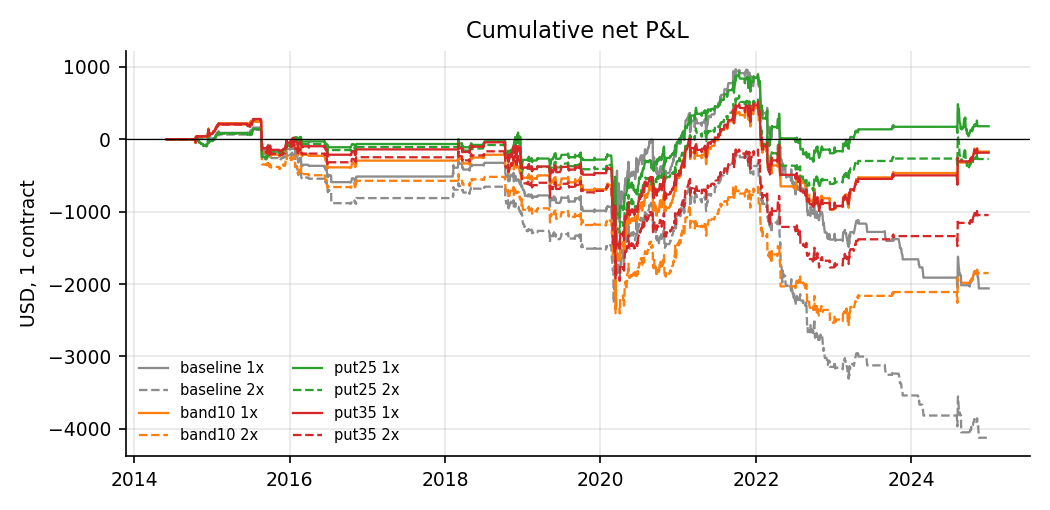
\includegraphics[width=0.92\linewidth]{figures/cum_pnl.png}\caption{Cumulative net P\&L, 1x solid and 2x dashed; baseline (live rules) grey}\end{figure}

\texttt{put25} (green) stays above the ATM book from 2016 on (from September 2015 at 2x). At 1x it ends 2019 at \ensuremath{-}\$280 (ATM \ensuremath{-}\$691), 2021 at +\$846 (+\$431) and 2022 at \ensuremath{-}\$194 (\ensuremath{-}\$974). At 2x the gap is wider: \ensuremath{-}\$617 against \ensuremath{-}\$2,532 at the end of 2022. Its lowest point is \ensuremath{-}\$1,085 at 1x (April 2020), against \ensuremath{-}\$1,748 for the ATM book (March 2020).

\begin{figure}[H]\centering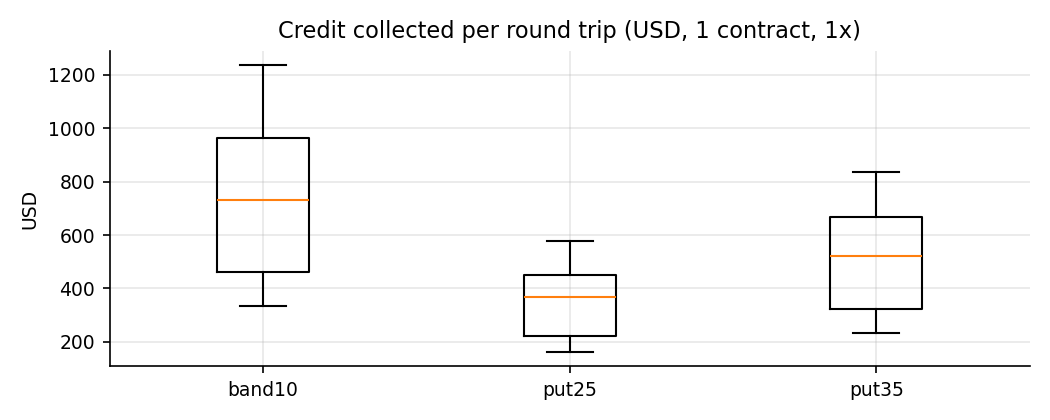
\includegraphics[width=0.92\linewidth]{figures/premium.png}\caption{Credit collected per round trip}\end{figure}

A 25-delta put collects about half the credit of the ATM put (median \$367 against \$731). So the stop (1x credit) and the 50\% profit-take are about half as far away in dollars.

\begin{figure}[H]\centering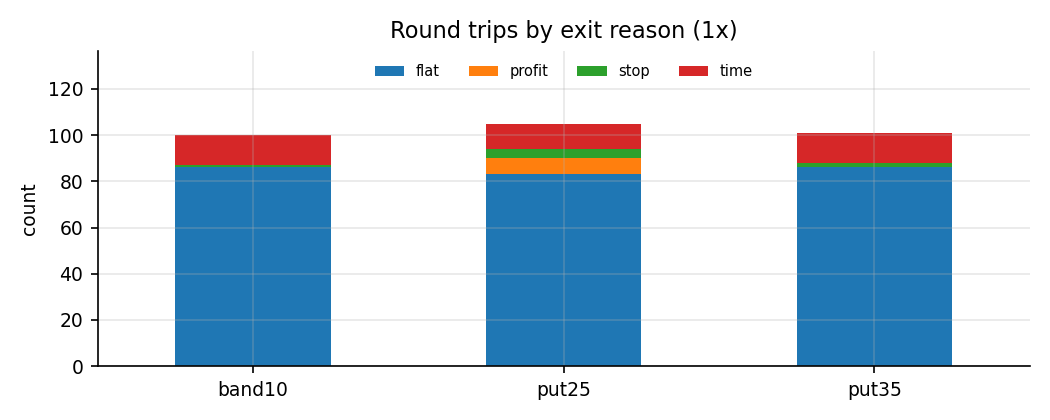
\includegraphics[width=0.92\linewidth]{figures/exits.png}\caption{Round trips by exit reason}\end{figure}

The smaller credit changes the exits. \texttt{put25} takes profit 7 times and is stopped 4 times; the ATM book took no profits and was stopped once. Most trades still close on the 3-day flat exit.

\begin{figure}[H]\centering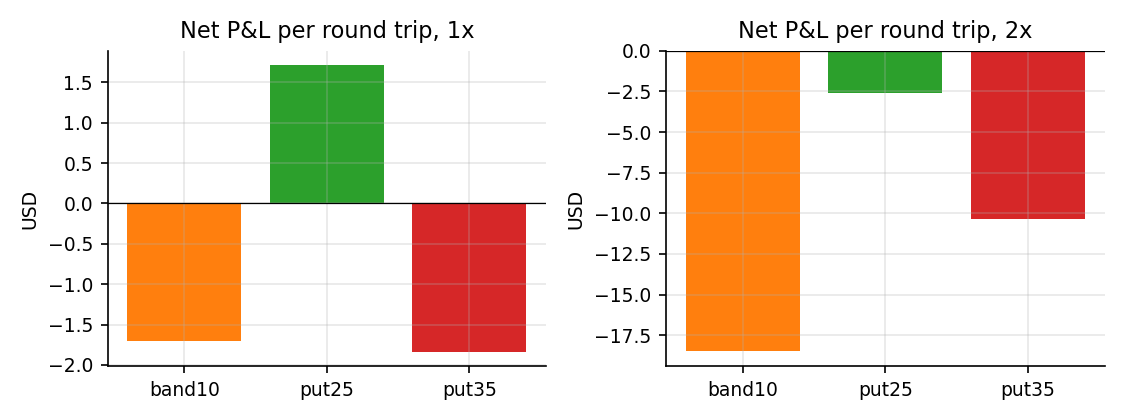
\includegraphics[width=0.92\linewidth]{figures/per_trade.png}\caption{Net P\&L per round trip}\end{figure}

Per round trip, \texttt{put25} is the only book above zero at 1x (+\$1.7). At 2x it loses \$2.6 per trip, against \$18.5 for the ATM book.

\begin{figure}[H]\centering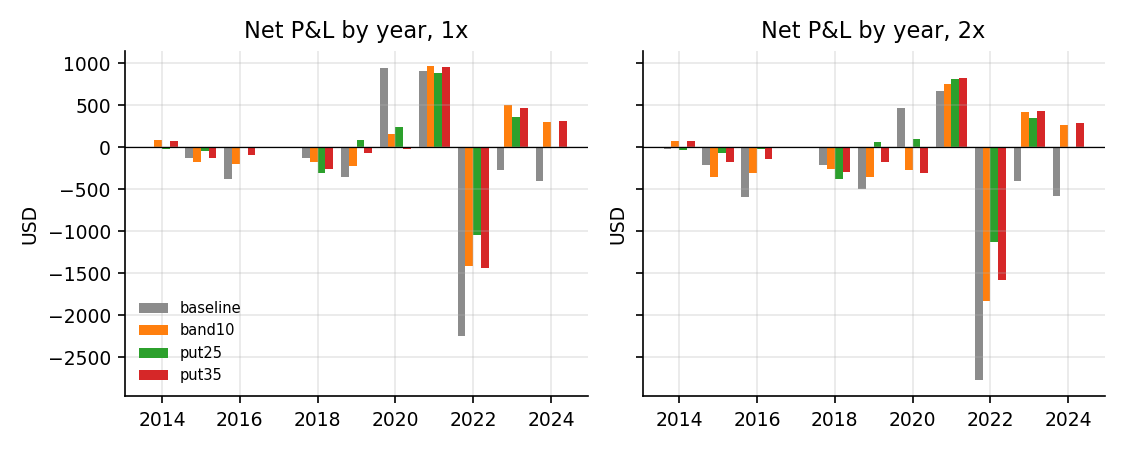
\includegraphics[width=0.92\linewidth]{figures/yearly.png}\caption{Net P\&L by year}\end{figure}

At 1x, \texttt{put25} beats the ATM book in 2015, 2016, 2019, 2020 and 2022 (+\$366), and trails in 2014, 2018, 2021, 2023 and 2024 (\ensuremath{-}\$748 together; 2017 is a tie with no trades). The 2020-2024 fail comes from 2023 and 2024 (\ensuremath{-}\$430 together), years in which the ATM put collected more. At 2x it trails only in 2014, 2018, 2023 and 2024.

\begin{figure}[H]\centering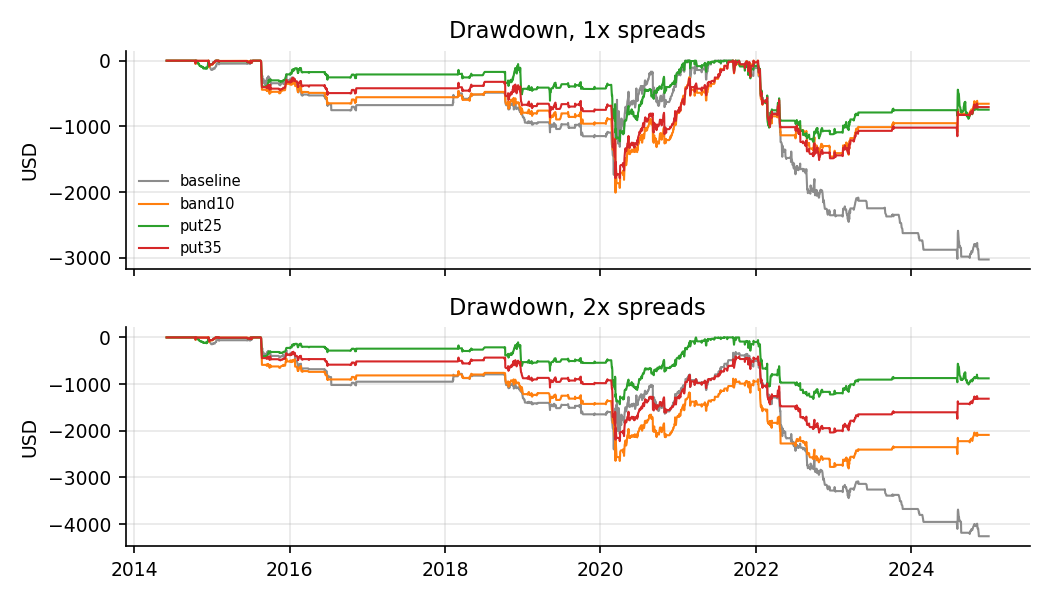
\includegraphics[width=0.92\linewidth]{figures/drawdown.png}\caption{Drawdown at 1x and 2x spreads}\end{figure}

The maximum drawdown falls from \$2,010 to \$1,237 at 1x, and from \$2,806 to \$1,431 at 2x.

\begin{figure}[H]\centering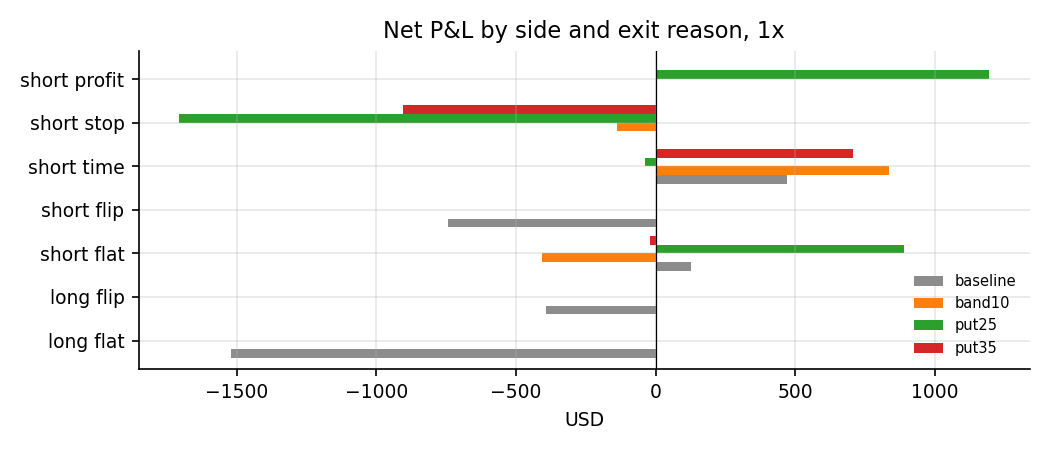
\includegraphics[width=0.92\linewidth]{figures/by_reason.png}\caption{Net P\&L by side and exit reason, 1x}\end{figure}

On the 25-delta book the flat exits make money (+\$889) and so do the profit-takes (+\$1,194). The four stops lose \$1,705.

\begin{figure}[H]\centering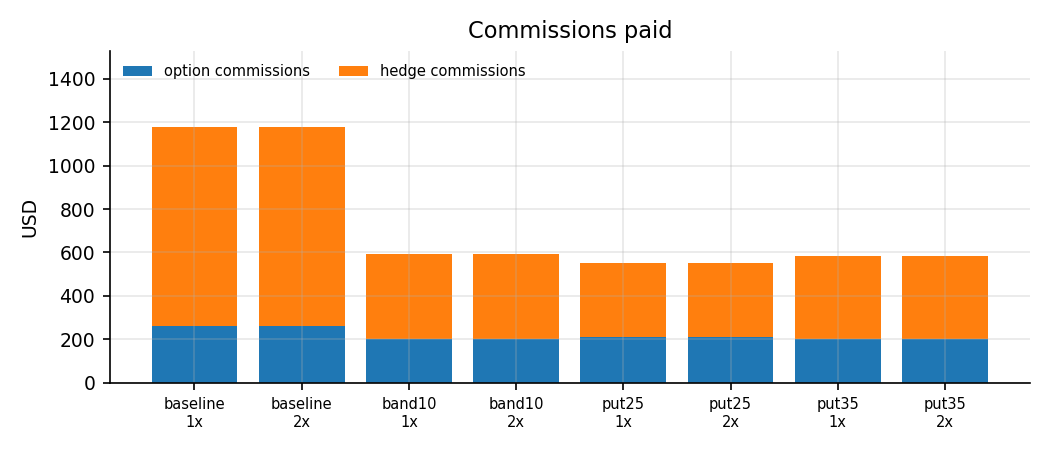
\includegraphics[width=0.92\linewidth]{figures/fees.png}\caption{Commissions paid}\end{figure}

Commissions fall slightly (\$550 against \$595), from fewer hedge orders: the position's delta is about half as large, so it drifts past the 10-share band less often.

\section{Analysis}

The hypothesis named a mechanism: out-of-the-money puts carry more premium per unit of risk. The data says the gain comes from somewhere else, so the reasoning needs correcting even though the result improved.

\begin{itemize}

\item \textbf{Before costs, the 25-delta book earns less, not more.} Net P\&L plus spreads plus commissions is +\$1,183 for \texttt{put25}, against +\$2,102 for the ATM book (0.56x). At entry the 25-delta put has about half the premium and delta of the ATM put on the same expiry, but about 0.8x its vega, 0.66x its gamma and the same theta. So the hedged volatility exposure falls only 20-35\%, while the edge before costs falls 44\%: the edge per unit of vega went down. The skew premium does not show up here.

\item \textbf{The whole gain is trading cost.} The spread cost (1x minus 2x equity P\&L) falls from \$1,677 to \$453. A cheaper option has a smaller spread in dollars. An out-of-the-money put also rarely ends deep in the money, where the spread model fits much wider closing costs. Commissions fall a little as well (\$595 to \$550).

\item \textbf{Edge per dollar of cost is what improved.} The ATM book spent \$2,272 in costs to earn \$2,102 before costs. The 25-delta book spent \$1,003 to earn \$1,183. That ratio is what turns the 1x result positive and nearly closes the 2x gap.

\item \textbf{The tail got smaller, but the stops got bigger.} The worst day falls from \ensuremath{-}\$727 to \ensuremath{-}\$399 (both on 2020-03-12), and ES from \ensuremath{-}\$87 to \ensuremath{-}\$72. But the four stops lose \ensuremath{-}\$1,705 together, the largest loss bucket in either book; the ATM book's one stop lost \ensuremath{-}\$138. An OTM put loses more as a multiple of its credit, and the 1x-credit stop sits closer in dollars.

\item \textbf{The 35-delta book does not sit neatly in between.} At 2x it does (\ensuremath{-}\$1,047), but at 1x it is slightly worse than the ATM book (\ensuremath{-}\$186 against \ensuremath{-}\$170). So the effect is not a smooth function of delta on this sample.

\end{itemize}

So the honest reading: selling further out of the money is a cheaper way to hold the same signal, not a richer source of premium. Most of the margin is mechanical cost reduction under the backtest's spread model, so it is only as good as that model. The one failed check is a \$60 shortfall in a half where both books made money, driven by two calm years.

\section{Verdict}

\textbf{Failed} on the pre-registered bar: 2020-2024 at 1x, by \$60. The bar is not changed after the fact, so this rule is not promoted. It is the strongest result in the desk's backtests so far: the only book with positive net P\&L over the full window at 1x, close to flat at 2x, with the smallest maximum drawdown.

Possible follow-ups, each needing its own card. Each is in-sample, and each adds trials:

\begin{itemize}

\item \textbf{Further out of the money (15-20 delta).} The cost argument predicts this helps again, until the fixed commission (\$2 per round trip) and the stop become large relative to a smaller credit.

\item \textbf{Two 25-delta contracts against one ATM contract.} This matches premium and delta, not vega (two contracts carry about 1.6x the ATM vega). It tests whether the cost advantage survives at the same premium collected.

\item \textbf{An OTM-put book as the new reference for later tests}, since it is now the cheapest structure.

\end{itemize}

\section{Caveats}

\begin{itemize}

\item \textbf{In-sample:} the idea comes from the PM's review of all 2026-10-16 results on this window.

\item \textbf{Spread model:} fitted on about two weeks of calm 2026 live quotes. The result rests on the model's cost difference between ATM and OTM puts, including its wider deep-in-the-money tier. That is the assumption most worth checking against real paper-account fills.

\item \textbf{Smile marks:} OTM put prices come from the per-expiry quadratic smile fit. The traded 25-delta strikes sit a median 4.0\% below spot (at most about 11\%), inside the fitted range (|ln K/\allowbreak{}F| up to 0.15).

\item \textbf{One contract:} the \$1 order minimum still applies to each hedge order. Month-end R2 days are missing (89 skipped times).

\item \textbf{Few stops:} the stop and profit-take effects rest on 4 and 7 events.

\end{itemize}

\section{Trials}

4 trials for this experiment (2 variants at 1x and 2x, one run of \texttt{experiment.\allowbreak{}py} at commit 06dbdc8), plus the baseline's 2. The reference was reused from \texttt{2026-\allowbreak{}10-\allowbreak{}16-\allowbreak{}short-\allowbreak{}only-\allowbreak{}band10} (2 trials, not rerun). After the run, the per-round-trip chart colours and the exit-chart legend were fixed and the figures were rebuilt with \texttt{-\allowbreak{}-\allowbreak{}report-\allowbreak{}only}, adding no trials. The pass bar was not changed.

\end{document}
